\chapter{Charged pion reconstruction and identification}
\label{ch:reconstruction}
\graphicspath{{Chapter-Reconstruction/figures/}}


\section{Tracking algorithm}

%% for general track fitting overview see:
%% http://www.phys.ufl.edu/~avery/fitting.html

\cite{Aad:2010bx} %% ID commisioning and calibration - good summary
\cite{Cornelissen:2007vba} %% ATLAS new tracking (NEWT)
\cite{Cornelissen:2008zza} %% global chi^2 track fitter

\section{Track reconstruction performance}

\begin{figure}[t]
  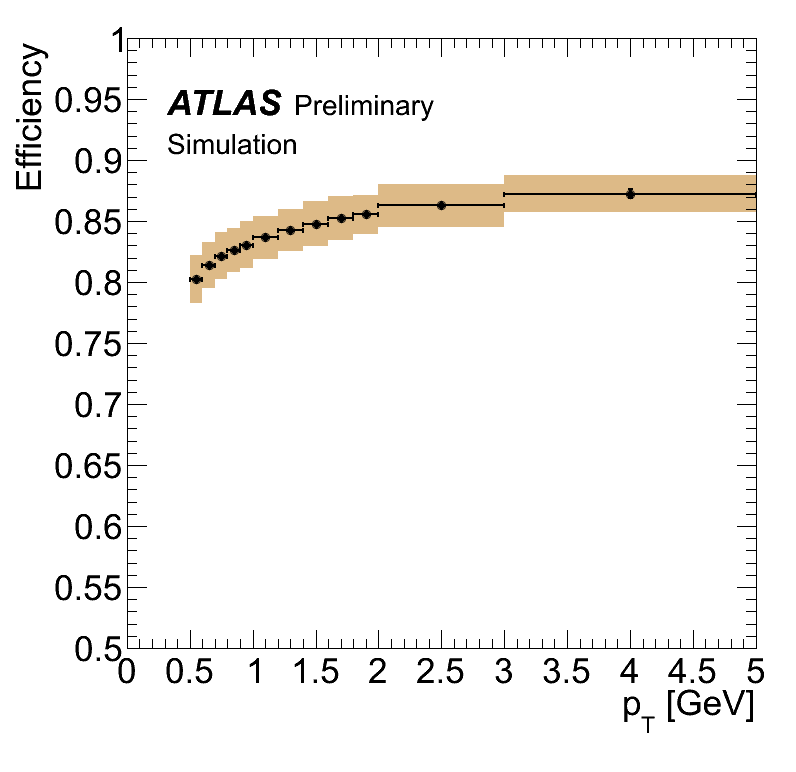
\includegraphics[width=0.49\linewidth]{atl_com_phys_2012_1541_fig_07_eff_pt.png}
  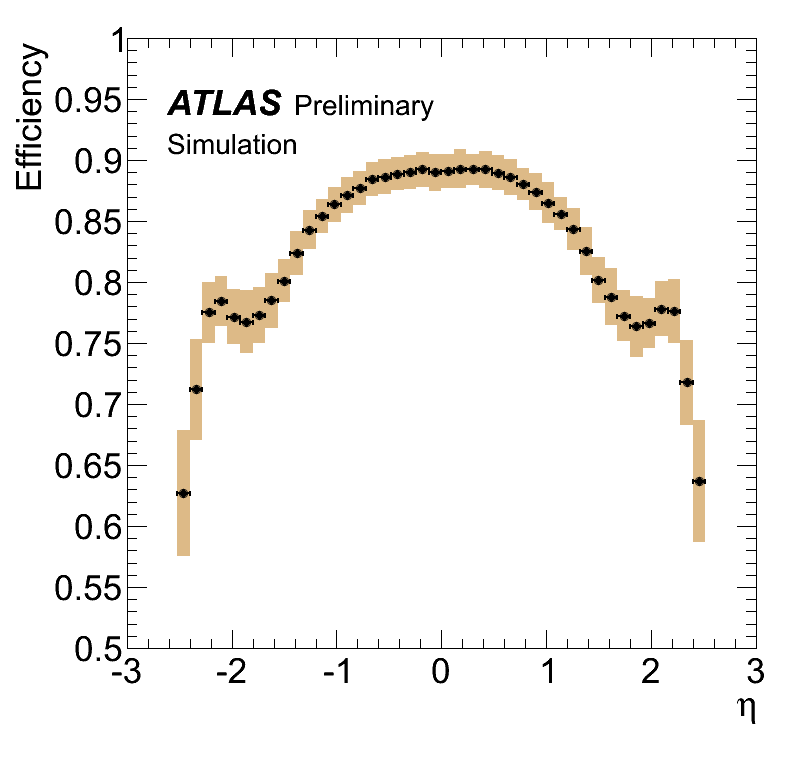
\includegraphics[width=0.49\linewidth]{atl_com_phys_2012_1541_fig_08_eff_eta.png}
  \caption{The Run-1 track reconstruction efficiency as a function of transverse momentum (left) and pseudorapidity (right).}
  \label{fig:trk_eff}
\end{figure}

\section{Pion identification}


